
\chapter{Image Registration Framework}\label{se:registration_framework}

\begin{flushright}
	\emph{Every working mathematician knows that if one does not control oneself (best of all by examples), then after some ten pages half of all the signs in formulae will be wrong and twos will find their way from denominators into numerators. \\ -V.I. Arnold}
\end{flushright}


% % % % % % % % % % % % % % % % % % % % % % % % % % % % % % % % % % % % % %
% % SUB SECTION
% % % % % % % % % % % % % % % % % % % % % % % % % % % % % % % % % % % % % %
\section{Introductory Definitions}
We define a \emph{$d$-dimensional image} as a continuous function from a subset $\Omega$ of the coordinate space $\mathbb{R}^{d}$ (having in mind particular cases $d=2,3$) to the set of real numbers $\mathbb{R}$. Given two of them  $T : \Omega_{T}  \rightarrow\mathbb{R} $ and $R : \Omega_{R}  \rightarrow\mathbb{R} $, called respectively \emph{target image} and \emph{reference image}, the \emph{image registration problem} consists in the investigation of features and parameters of the transformation function
\begin{align*}
\varphi :\mathbb{R}^{d} \supseteq \Omega_{R} & \longrightarrow \Omega_{T}\subseteq \mathbb{R}^{d}   \\
\mathbf{x} &\longmapsto \varphi (\mathbf{x}) 
\end{align*}
such that for each point $\mathbf{x}\in \Omega_{t} $ the element $T(\varphi (\mathbf{x}))$ and $R(\mathbf{x})$ are closed as possible according to a chosen metric. 
The underpinning idea can be represented by the following diagram, where $\varphi$ is the solution that makes $f$ the identity function.

\[
\begindc{\commdiag}[40]
\obj(-30,30)[Or]{$\Omega_{R}$}
\obj(0,30)[Ot]{$\Omega_{T}$}
\obj(-30,10)[Rref]{$\mathbb{R}$}
\obj(0,10)[Rtarg]{$\mathbb{R}$}

\mor{Or}{Ot}{$\varphi$}
\mor{Or}{Rref}{$R$}
\mor{Ot}{Rtarg}{$T$}
\mor{Rref}{Rtarg}{f}[1,1]

\enddc
\]
% fine diagramma

\noindent
This definition leave two degrees of freedom in searching for a solution: the domain of the transformation (also called deformation model), and the metric to measure the similarity between images. \\
Once these are chosen, they can be used as constituent of an \emph{image registration framework}: an iterative process that at each step provides a new function $\varphi$ that approaches $f$ to the identity (figure \ref{fig:iterative_algorithm_scheme}).
\begin{figure}[!ht]
	\centering
	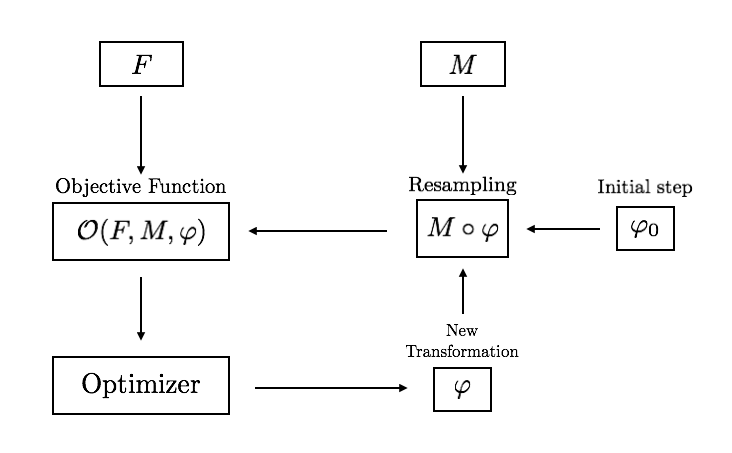
\includegraphics[scale=0.35]{figures/iterative_algorithm.png}
	\caption{Generic image registration framework scheme.}
	\label{fig:iterative_algorithm_scheme}
\end{figure}
This framework can provide additional degrees of freedom: the metric can be considered with an additive regularization term, that introduces a constraint based on prior knowledge about the searched solution:
\begin{align*}
\mathcal{O}(R,F\circ\varphi) = \text{Sim}(R,F,\varphi) + \mathcal{R}(\varphi) 
\end{align*}
where Sim is a function to measure the similarity while $\mathcal{R}$ is the regularization term.
In addition optimization algorithm on which the optimizer is based and the resampling (the process of resize the image from one dimension to another) strategy can be defined over several possibilities.
This generic scheme is far from being fixed and among all of the possible degrees of freedom there can be several variants (for a survey in image registration see for example \cite{Sotiras:survey:13}, \cite{Hill:survey:01}). Moreover each of the implementation currently available may have been performed in different ways according to the authors need and perspective.\\
%Since the implementations that accompany this research are based on NiftyReg (BIBLIOREF) software, a scheme of this particular case can be found in the appendix.\\
In this thesis $\varphi$ will be bounded to the group of rigid transformation or in the set of bijective continuous function with continuous inverse (i.e. diffeomorphisms).
Using diffeomorphisms with the underpinning Lie algebra and Lie group theory was proposed for the first time in 2006 (Arsigny et Al \cite{Arsigny:MRM:06}), as a faster improvement to the affine invariant Riemannian approach, has found successful applications in many domains of medical imaging (in vivo mosaicing \cite{Vercauteren:PHD:08}, brain Alzheimer detection \cite{Lorenzi:PhD:12}, cardiac image analysis \cite{Mansi:IJCV:11}, mandible imaging using polyaffine registration \cite{Seiler:MICCAI:11}) and has been continuously improved since its introduction (Ashburner \cite{Ashburner:07}, Vercauteren \cite{VercauterenPPA08}, Lorenzi \cite{Lorenzi:pt:13}). In this setting, computations in the Lie group of diffeomorphism are made in its Lie algebra, in which it is possible to apply easily calculus and statistics.


% % % % % % % % % % % % % % % % % % % % % % % % % % % % % % % % % % % % % %
% % SUB SECTION
% % % % % % % % % % % % % % % % % % % % % % % % % % % % % % % % % % % % % %
\section{Iterative Registration Algorithm}



% % % % % % % % % % % % % % % % % % % % % % % % % % % % % % % % % % % % % %
% % SUB SECTION
% % % % % % % % % % % % % % % % % % % % % % % % % % % % % % % % % % % % % %
\section{Using Diffeomorphisms: Utility and Liability}




% % % % % % % % % % % % % % % % % % % % % % % % % % % % % % % % % % % % % %
% % SUB SECTION
% % % % % % % % % % % % % % % % % % % % % % % % % % % % % % % % % % % % % %
\subsection{Parametrization of Diffeomorphisms: LDDMM and SVF}




% definition of svf


% % % % % % % % % % % % % % % % % % % % % % % % % % % % % % % % % % % % % %
% % SUB SECTION
% % % % % % % % % % % % % % % % % % % % % % % % % % % % % % % % % % % % % %
\subsection{Composition of Diffeomorphisms: the BCH formula}














Among multiple approaches in image registration, the use of diffeomorphism 


Under this light, the transitions from the Lie group to Lie algebra (the Lie logarithm) and its return (the Lie exponential) become fundamental tools.
The main topic of this research is the evaluation of the operation that we define here as \emph{Lie algebra Group Composition}, or simply \emph{Group Composition}, defined as the vector $\mathbf{w}$ in the Lie algebra $\mathfrak{g}$ that reflects the composition in the Lie group of two vectors $\mathbf{u}, \mathbf{v}$ in the same tangent space:
\begin{align*}
\mathbf{w} = \log(\exp(\mathbf{u})\circ\exp( \mathbf{v}))
\qquad
\forall \mathbf{u}, \mathbf{v} \in \mathfrak{g}
\end{align*}
The role that the Group Composition plays in the diffeomorphic image registration is presented in the next subsection and explored in a formal way in section \ref{se:log_composition}.










The definition of the registration problem and the iterative algorithm described raise several issues. For example there are no reasons to believe that such a correspondence is unique and that there is at least one of them whose behaviour corresponds to a reasonable biological transformation between anatomies. 
Some constraints on $p$ must be defined in order to have a transformation that models realistic changes that can occur in biological tissues.
The kind of constraint that we will use in this research is to give some limitation to set (and the consequent mathematical structure) in which the transformation $p$ lives.\\
In the finite dimensional case a big family of transformation suitable for $p$ is given by the category of the complete subgroup of $\text{GL}(d)$, called Matrix Lie group, or Classical Lie group.
One of the Matrix Lie group explored in this research is the special euclidean group $\text{SE}(d)$, or group of rigid transformations.
A little increase in the number of degrees of freedom leads to the group of the affine transformations, where scaling and shearing have been added to the possible transformations. \\
The idea of maximize the number of degrees of freedom in a transformation that maintains anatomical features between images, led to consider the Lie group of diffeomorphism $\text{Diff}$.
A diffeomorphism $p$ can be expressed as the sum of the identity function with a differentiable transformation depending on $\mathbf{x}$. It is possible to write:
\begin{align*}
p(\mathbf{x})  = \mathbf{x} + \gamma(\mathbf{x})
\end{align*}
With this notation the vector $\dot{\gamma}(\mathbf{x})$ is the speed\footnote{as we will see, a feasible way to express a set of diffeomorphisms is as the solution of the differential equation defined by the velocities of the transformation.} of each point from its original to a new position due to the application of $p$.\\
In the iterative diffeomorphic registration algorithm (in which the structure is defined by regularization and similarity), to obtain the update at each step, it is required to apply consecutively two diffeomorphisms $p_{i}$ and  $\hat{p}_{i+1}$ and consider the resulting composition as the required update.
%\begin{figure}[!ht]
%	\centering
%	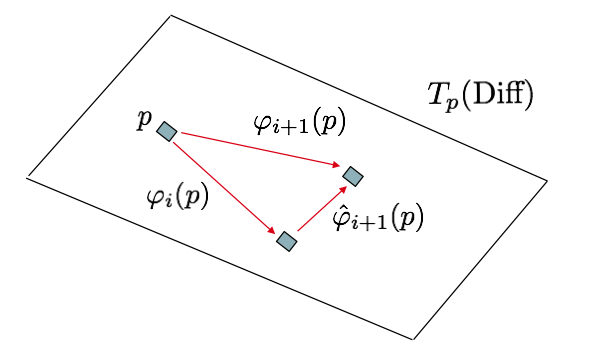
\includegraphics[scale=0.35]{figures/diff_update.png}
%	\caption{Composition of tangent vectors of diffeomorphism (provisional).}
%	\label{fig:composition1}
%\end{figure}
As a consequence, the corresponding vector of the transformation $p_{i+1}$ in the tangent space of the Lie group can be computed, given two vectors in the tangent bundle, with an operation called here \emph{the group composition in the Lie algebra}.\\
In \cite{Bossa2007} the BCH formula appears as an improvement of the scaling and squaring algorithm to compute the logarithm of a matrix. As noticed in the same paper, the BCH formula is used in a infinite dimensional settings, while its validity has been proven only for finite dimensional Lie group. In addition while composing the logarithm of a composition of two exponentials, the initial tangent vectors belongs to the same tangent space. This is not the case while composing $p_{i}$ with $\hat{p}_{i+1}$ the tangent vector that defines $\hat{p}_{i+1}$ is an element of the tangent plane to $p_{i}$. \\
Is it possible to reach a proper computation thanks to the definition of Affine exponential, that differs from the Lie exponential used in \cite{Bossa2007} .






The BCH formula provides an expression of the Group Composition in the finite dimensional case expressed as an infinite series of nesting commutators. The difficulties involved in dealing with this formula, as well as its non completely proper use in the infinite dimensional setting, gave birth to some methodologies and approaches, whose investigation is the main goal of this research. One of these approaches, involves the Taylor expansion and has a computable form in the finite dimensional. A geometrical approach that holds also in the infinite dimensional case is the parallel transport.
It can be considered as a natural approach to evaluate the group composition with offset. It consists in the transport of the vector $\mathbf{v}$ along the geodesic having $\mathbf{u}$ as tangent vector such that during the transport it maintains the condition of parallelism. The resulting vector $\mathbf{v}^{\parallel}$ in the tangent plane of $\mathbf{u}$ can be then summed with $\mathbf{v}$ with similar results to the direct application of the BCH. Its evaluation involves the Schild's ladder and the pole ladder. Both have already found practical application in medical imaging \cite{Lorenzi:discrete_ladders:14}, \cite{Lorenzi:pt:13}.
Parallel transport is necessarily related with the definition of the connection. Choosing among possible connections become a crucial feature, whose consequences in the corresponding realization in the transformation of images requires further studies.

\begin{figure}[!ht]
	\centering
	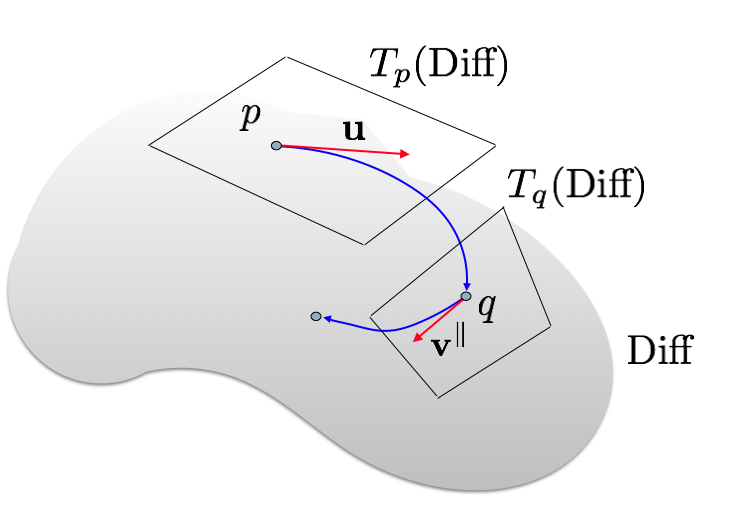
\includegraphics[scale=0.25]{figures/parallel_transport_1.png}
	\caption{Group composition with offset using parallel transport.}
	\label{fig:composition}
\end{figure}

The lack of a close form of any kind and the theoretical difficulties inherent to the investigation of infinite dimensional group of diffeomorphism makes an experimental approach meaningful. 











